\chapter{\IfLanguageName{dutch}{Stand van zaken}{State of the art}}
\label{ch:stand-van-zaken}

% Tip: Begin elk hoofdstuk met een paragraaf inleiding die beschrijft hoe
% dit hoofdstuk past binnen het geheel van de bachelorproef. Geef in het
% bijzonder aan wat de link is met het vorige en volgende hoofdstuk.

% Pas na deze inleidende paragraaf komt de eerste sectiehoofding.

\section{Personalisatie}
\label{sec:Personalisatie}

Personalisatie van webapplicaties en websites draait erom de bezoekers een op maat gemaakte ervaring aan te bieden. Dit kan op verschillende manieren toegepast worden, en kan meerdere doelen hebben. 

In dit hoofdstuk wordt er verder ingegaan op welke manieren personalisatie van websites hedendaags wordt toegepast, en wat dit betekent voor zowel de bezoeker als het bedrijf zelf.

\subsection{Personalisatie op basis van e-mail en sociale media}
\label{subsec:Personalisatie op basis van e-mail en Social Media}

Zowat iedereen heeft wel te kampen met een overvloed aan e-mails in hun postvak van allerlei websites waar ze hun e-mailadres ooit hebben vrijgegeven. Het is een courante denkwijze om er van uit te gaan dat deze  e-mails door de meeste mensen simpelweg verwijderd worden, maar e-mailmarketing blijft een van de meest succesvolle marketingstrategieën \autocite{Dehkordi2012}. 

E-mailmarketing is relatief makkelijk te implementeren en vereist weinig technische investering, meestal wordt dit verwezenlijkt via systemen van derden zoals bijvoorbeeld \href{https://mailchimp.com/}{MailChimp}. 

Een nadeel van deze marketingvorm is dat het bedrijf continu bezig moet zijn met nieuwe inhoud te creëren voor deze e-mails, ook moet de website continu geüpdatet worden met relevante informatie en pagina's die relevant zijn voor de e-mails die ze versturen.

\subsection{Personalisatie op basis van geografische locatie}
\label{subsec:Personalisatie op basis van geografische locatie}

Geografische personalisatie is het aanpassen van de website op basis van de locatie van de gebruiker. Gebruikers uit België die naar de website van een internationaal bedrijf surfen, zullen dan worden omgeleid naar een Nederlandse of Franse versie van die website.

Geografische personalisatie kan ook gebruikt worden om de inhoud van een pagina aan te passen aan de hand van de locatie van de gebruiker, of om vertalingen aan te bieden.

Een nadeel hiervan is dat mensen die op reis gaan het soms moeilijk zouden kunnen hebben om naar de juiste versie van de website te navigeren, aangezien het systeem de gebruiker zal willen omleiden naar de pagina of inhoud die voorzien is voor het land waar zij zich momenteel in bevinden. Eenzelfde probleem kan zich voordoen bij bedrijven die hun webverkeer omleiden via een ander land door middel van bijvoorbeeld een VPN. 

Een mogelijke oplossing voor dit probleem is het bijhouden van cookies. Als de geografische informatie over een gebruiker daarin wordt opgeslagen, kan deze via de cookie opgehaald worden en zal een gebruiker alsnog de website met de correcte inhoud en taal aangeboden kregen. Als de gebruiker geen cookies toelaat, of zijn cookies verwijdert, wordt deze mogelijke oplossing tenietgedaan.

Geografische personalisatie is ook relatief eenvoudig te implementeren en kan een grote troef zijn op de internationale markt. 

\subsection{Personalisatie op basis van IP-adres}
\label{subsec:Personalisatie op basis van IP-adres}

Deze methode van personalisatie is wat minder opvallend, aangezien het bij de gemiddelde internetgebruiker weinig tot nooit zal voorkomen, dit omdat zij het internet gebruiken via een serviceprovider zoals Telenet of Proximus. 

Deze vorm van personalisatie wordt gebruikt om zakelijke gebruikers en bedrijven te kunnen identificeren op basis van hun IP-adres. Zo kan men zien of een bezoeker bij een bepaald bedrijf werkzaam is om deze direct aan te spreken op bijvoorbeeld de homepagina.

\begin{figure} [hbt!]
	\centering
		
\includegraphics[width=\linewidth]{img/IP-based-personalization}
\caption[Personalisatie op basis van IP adres]{ Personalisatie op basis van IP adres}
		\floatfoot{Source: https://www.optimizely.com/optimization-glossary/account-based-marketing/} 
	\label{fig:IPBasedPersonalization}
\end{figure}


Net zoals bij personalisatie op basis van locatie kan dit misleidende resultaten opleveren, bijvoorbeeld als de werknemer van thuis werkt of het IP-adres niet duidelijk aantoont vanuit welk bedrijf het webverkeer van de bezoeker afkomstig is. Ook voor performantie kan dit negatieve gevolgen hebben, aangezien deze vorm van personalisatie afhankelijk is van systemen van derden. 

Verder moet er ook inhoud gecreëerd worden voor elk bedrijf dat men specifiek wil aanspreken. Dit is een tijdrovend proces, maar aangezien deze vorm van personalisatie weinig voorkomt, is het wel een troef waardoor het bedrijf zich kan onderscheiden van de meerderheid en zich kan laten opvallen.

  
 \subsection{Verwante inhoud personalisatie}
 \label{subsec:Verwante inhoud personalisatie}
 
 Dit is de vorm van personalisatie die een grote meerwaarde zal leveren aan dit onderzoek. De meeste mensen hebben deze vorm al ondervonden op een webshop zoals Amazon of Bol.com. Deze vorm van personalisatie draait erom de gebruikers artikels of producten aan te raden op basis van items die ze al eerder bekeken hebben, alsook het gedrag van andere gebruikers.
 
De werking van het aanbevelingssysteem van Amazon is gebaseerd op enkele complexe algoritmen. \autocite{Linden2003} Dit is natuurlijk verantwoord omdat zij een gigant zijn in de e-commerce industrie. Amazon werkt op zeer grote schaal en heeft veel geld geïnvesteerd in de ontwikkeling van hun systeem. 

\newpage
In de realiteit hoeven de technologieën voor aanbevelingen van producten niet zo complex te zijn voor gewone webshops en bedrijven, vaak is het voldoende om relaties te creëren tussen artikels en op basis van deze relaties nieuwe artikels aan te raden aan de gebruikers. 

Een voorbeeld van een relatie tussen twee artikels is de welbekende 'Anderen bekeken ook' blok die vaak zichtbaar is bij het bekijken van een detailpagina van een product. 

Een simpelere methode van dergelijke relaties is het aanbieden van verwante producten op basis van categorieën of tags. Tags zijn een manier om kenmerken van een product weer te geven die specifieker zijn dan een categorie. Een categorie kan dan 'schoenen' zijn, terwijl een tag 'lage sneakers' is. 

Dit is een klassiek voorbeeld van de probleemstelling van dit onderzoek. De zoekfunctie is dus beperkt tot de productcatalogus en de informatie die beschikbaar is over deze producten. De website maakt dus geen gebruik van persoonlijke informatie om deze zoekresultaten te personaliseren.

Over de mogelijkheden van het personaliseren van zoekresultaten gaan we dieper in in het volgende hoofdstuk van deze literatuurstudie.

 \subsection{Personalisatie op basis van gebruikersprofiel}
\label{subsec:Personalisatie op basis van gebruikersprofiel}

Net zoals bij personalisatie op basis van IP adres, waar een bedrijf de inhoud die ze aanbiedt op haar website aanpast naargelang welk bedrijf er naartoe surft, kan er per individuele gebruiker andere inhoud getoond worden. 

Een voorbeeld hiervan is dat klant A andere promo's te zien zal krijgen dan klant B, afhankelijk van de informatie die over deze twee personen beschikbaar is. Een persoon die bijvoorbeeld enkel voor telefonie klant is bij een telecombedrijf, zal eerder promo's krijgen voor pakketten waar telefonie gecombineerd wordt met een ander product.

Deze vorm van personalisatie is enkel mogelijk wanneer de gebruiker een account heeft aangemaakt bij een bepaalde website, zodat er geweten kan zijn van welke producten deze klant reeds gebruik maakt. Dit brengt ons dichter bij het gebied van aanbevelingssystemen, wat uitvoerig besproken zal worden in het volgende hoofdstuk.

\section{Recommender Systems}
\label{sec:Recommender Systems}
Recommender Systems \autocite{Resnick1997} zijn aanbevelingen vanuit het systeem die rekening houden met de beschikbare informatie van gebruikers en hun voorkeuren om zo een filter te plaatsen op de informatie die weergegeven wordt. Verder zullen we deze benoemen aan de hand  van hun Nederlandse naam 'aanbevelingssystemen'.

Aanbevelingssystemen worden vooral gebruikt in e-commerce toepassingen waar een zeer groot en verscheiden aanbod aan producten is, en het al vaak lastig wordt om precieze aanbevelingen aan de klant te geven. Hierbij wordt allerlei informatie van een gebruiker verzameld, zoals historische aankopen, items op het verlanglijstje, items waar de gebruiker op geklikt heeft, etc.

In dit onderdeel zullen we kort wat dieper ingaan op de werking van dergelijke aanbevelingssystemen en de achterliggende algoritmen.

\subsection{Haalbaarheid}
\label{sec:Haalbaarheid}

Een degelijk systeem biedt een grote meerwaarde voor een bedrijf, zo heeft Netflix een competitie gehouden die 1 miljoen dollar bood aan degene die een aanbevelingssysteem kon maken dat 10\% beter presteerde dan hun bestaande systeem. 

Deze wedstrijd liep van oktober 2006 tot minstens oktober 2011. De wedstrijd werd de \cite{NetflixPrize} genoemd, Netflix stelde hiervoor een dataset beschikbaar. Enkele groepen hebben het doel behaald, maar het algoritme van de winnende groep is uiteindelijk nooit in productie gebracht, omdat de mogelijke opbrengst niet kon opwegen tegen de extra gevraagde rekenkracht. 

Een aanbevelingssysteem moet dus niet enkel de juiste waarden kunnen aangeven, het moet ook realistisch en haalbaar zijn qua rekenkracht en extra bijkomende kosten voor onderhoud. Het ontwerpen van dergelijk systeem is dus geen eenvoudige klus.

\subsection{Algoritmen voor aanbevelingssystemen}
\label{sec:Algoritmen voor aanbevelingssystemen}

We spreken over twee grote categorieën in algoritmen van aanbevelingssystemen: 'collaborative filtering'-algoritmen en 'content based'-algoritmen.  \autocite{Adamovicius2005} Door de evolutie en groeiende ontwikkeling van beter presterende systemen zijn er ondertussen ook enkele algoritmen die niet echt binnen een van deze twee koepels vallen. In de onderstaande figuur wordt een simpele representatie gegeven van de werking van deze soorten algoritmes.

\begin{figure} [h!]
	\centering
	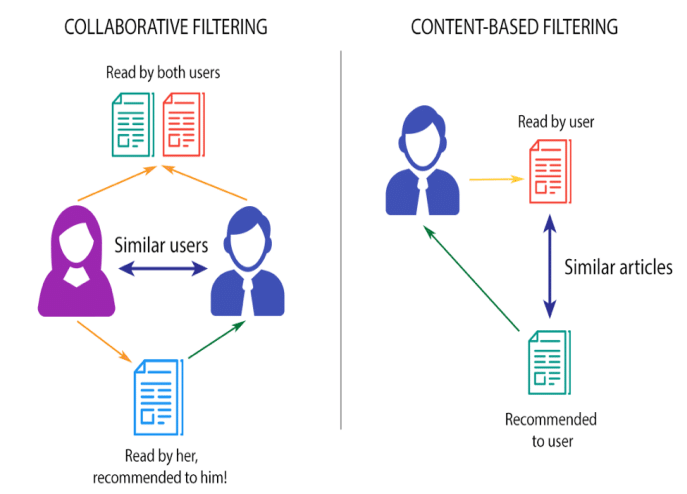
\includegraphics[width=\linewidth]{img/Content-based-filtering-and-Collaborative-filtering-recommendation}
	\caption[Vergelijking Collaborative Filtering - Content-Based Filtering]{Vergelijking Collaborative Filtering - Content-Based Filtering}
	\floatfoot{Source: https://www.researchgate.net/figure/Content-based-filtering-vs-Collaborative-filtering-Source\_fig5\_323726564} 
	\label{fig:CollaborativeVsContentBased}
\end{figure}
\newpage

	
\subsubsection{Collaborative Filtering}
\label{sec:Collaborative Filtering}

Het kernidee bij Collaborative Filtering \autocite{Schafera} is om aanbevelingen te maken gebaseerd op de voorkeuren van een andere gebruiker met een gelijkaardig gedrag. Zoals de figuur hierboven aantoont dat als gebruiker 1 en 2 hetzelfde artikel gelezen hebben, gebruiker 2 een artikel als aanbeveling zal krijgen dat gelezen werd door gebruiker 1. 
Hetzelfde idee kan toegepast worden op allerlei interacties van de gebruikers met een website zoals likes, shares, verlanglijstjes, etc.

In de praktijk geeft deze techniek zeer goede resultaten, maar zoals verwacht brengt dit ook enkele problemen met zich mee. Een eerste merkwaardig probleem is een zogenaamde cold start, dit komt onder andere voor bij de eerste interactie van een nieuwe gebruiker met een applicatie die aanbevelingen biedt. Het algoritme heeft dan onvoldoende informatie om een correcte en nuttige aanbeveling op te leveren aan de gebruiker. Een andere oorzaak voor dit cold-start fenomeen kan zijn dat er een nieuw product wordt toegevoegd aan het systeem, er kan dan nog niet geweten zijn welk type gebruiker hierin geïnteresseerd zou kunnen zijn. 

\newpage
Een tweede probleem die het succes van een Collaborative Filtering algoritme negatief kan beïnvloeden is het aantal gebruikers van een systeem. Met andere woorden, hoe meer gebruikers er zijn, hoe correcter de aanbevelingen aan een specifieke gebruiker zal zijn. \autocite{Sarwar2001}. Een gebruiker met ongewone interesses zal logischerwijs in een klein systeem weinig gelijkaardige gebruikers hebben, en zal dus ook geen optimale aanbevelingen krijgen.

Een groot voordeel van Collaborative Filtering is dat er absoluut geen kennis hoeft te zijn van de toepassing van het systeem, de aanbevelingen worden gegenereerd op basis van het gedrag van de gebruikers en zijn interesses. De producten of hun attributen moeten dus niet gekend zijn om aanbevelingen te kunnen geven, dat maakt het eenvoudiger om een aanbevelingssysteem met de techniek van Collaborative Filtering te implementeren.

\subsubsection{Content Based}
\label{sec:Content Based}

Content Based aanbevelingssystemen \autocite{Lops2011} maken, in tegenstelling tot Collaborative Filtering, wel gebruik van de specifieke producten binnen het systeem en hun attributen. Op basis van deze attributen en de interesse van de gebruiker daarin, wordt per gebruiker een profiel opgezet, elk attribuut krijgt dan een score toegekend, een hogere score betekent grotere interesse. Een attribuut van een product kan dan bijvoorbeeld 'schoenen' of 'PS4 games' zijn, of zelfs een filmgenre.

Een eerste probleem bij Content Based algoritmen is, net zoals bij Collaborative Filtering, het cold start probleem. Als een nieuwe gebruiker het systeem gebruikt, is er voor deze gebruiker nog geen profiel opgesteld en kunnen er ook geen aanbevelingen gemaakt worden.

Een tweede probleem van Content Based algoritmen wordt overspecialisatie genoemd, dit treedt op wanneer het systeem eigenlijk té accurate aanbevelingen doet. Het gevolg hiervan is dat slechts enkele producten voldoen aan de verwachtingen van het systeem, waardoor er geen nieuwe aanbevelingen aan de gebruiker naar voor gebracht worden, en de gebruiker enkel producten zal zien die hij reeds bekeken heeft. 

Een derde probleem bij Content Based algoritmen treedt op wanneer producten slecht gelabeld zijn, en hun attributen onvoldoende passen bij wat het product effectief is. Hierdoor kan het systeem deze producten niet goed vergelijken met andere. Dit is vooral een probleem wanneer de attributen van de producten van verschillende bronnen afkomstig zijn, of manueel slecht opgesteld zijn.

Het probleem bij Collaborative Filtering algoritmen waar bij het toevoegen van nieuwe producten niet geweten kan zijn welke gebruikers hierin geïnteresseerd zouden zijn, is niet van toepassing bij Content Based algoritmen. Het systeem maakt gebruik van de attributen van producten, dus nieuwe producten kunnen meteen belanden in de aanbevelingen van gebruikers die reeds interesse getoond hebben in andere producten met die attributen. Ook het aantal gebruikers binnen een systeem vormt om dezelfde reden geen probleem bij Content Based aanbevelingssystemen. 


\subsubsection{Hybrides}
\label{sec:Hybrides}

Beide van de voorgenoemde technieken hebben elk hun eigen voor- en nadelen, alsook sterke en zwakke punten. Content Based heeft te kampen met overspecialisatie, maar is wel in staat om nieuwe producten meteen aan te bevelen aan de gebruikers. Collaborative Filtering heeft moeite met het aanbevelen van nieuwe producten en een cold start, maar heeft geen problemen in de aard van overspecialisatie.

De logische redenering is dan natuurlijk om deze twee soorten systemen te gaan combineren, kwestie van het beste van twee werelden te proberen bekomen. Dit worden hybride aanbevelingssystemen \autocite{Cano2017} genoemd.

De manier van het opbouwen van een hybride systeem kan zijn dat beide methoden afzonderlijk worden uitgevoerd, en hun resultaten op het einde samengebundeld worden. Dit is de meest eenvoudige implementatie.

Een andere manier van combineren kan zijn door de informatie binnen een Collaborative Filtering systeem aan te vullen met informatie uit de gebruikersprofielen. Hierdoor wordt de gelijkaardigheid van twee producten bepaald door zowel de inhoud en welke soorten typische gebruikers deze producten bekijken, kopen, leuk vinden, etc.
De informatie van deze gebruikers kan dan bijvoorbeeld leeftijdsgroep, woonplaats, gezinssamenstelling, etc. voorstellen.


\section{Wat is Graph?}
\label{sec:wat is Graph?}

In de context van deze bachelorproef zal er met 'Graph' steeds verwezen worden naar een Graph databank. In dit onderdeel zullen we wat dieper ingaan op wat dit soort databank precies inhoudt om een volledig begrijpen van de precieze werking te verzekeren. 

\subsection{Graph}
\label{sec:Graph}

Graph is de databankstructuur die verder in dit onderzoek gebruikt zal worden. Deze structuur maakt gebruik van een wiskundige graaf om data op te slaan. Een graaf bestaat uit een aantal knopen (genaamd nodes) die al dan niet verbonden zijn. 

\begin{figure} [ht]
	\centering
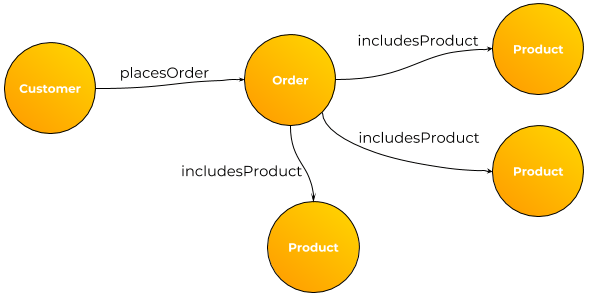
\includegraphics[width=\linewidth]{img/Customer-Order-Example-Graph.png}
	\caption[Voorbeeld Graph model]{Voorbeeld Graph model}
	\floatfoot{	Source: https://medium.com/@6point6ltd/use-cases-for-graph-databases-37ceb4903edd}
	\label{fig:GraphModelExample}
\end{figure}


Relaties hebben de prioriteit bij een graph databank, dit betekent dat relaties tussen knopen gepersisteerd worden in de databank, en niet enkel tijdelijk berekend voor een enkele query, dit is de reden waarom er geen complexe JOIN query's of foreign keys nodig zijn.

Graph databanken hebben dus een voordeel voor functionaliteiten zoals netwerken, aanbevelingen, etc. maar ook fraudedetectie. 

\subsubsection{Voordelen}
\label{subsec:Voordelen Graph}

Een groot voordeel van de graafstructuur die deze databanken gebruiken is dat deze sneller zijn dan relationele databanken omdat ze op zeer korte tijd naar een bepaalde node kunnen verwijzen, waarbij we bij een relationele databank een JOIN zouden moeten gebruiken. 

Graph databanken zijn ook zeer flexibel in gebruik. Bij het veranderen van een model kan er steeds verder gebouwd worden op het bestaande model, zonder dat hierdoor reeds verwezenlijkte functionaliteiten verloren zou kunnen gaan.
Dit is ook een voordeel bij het opstarten, er moet niet op voorhand grondig gediscussieerd worden over hoe het model er uiteindelijk uit zal moeten zien.

Deze troeven zijn niet te vinden bij traditionele databankstructuren die met tabellen werken, daarbij moet er alvorens het opzetten van de databank al een zekerheid zijn van hoe het model eruit zal zien, want het model zal de mogelijke functionaliteiten bepalen. Als er dan achteraf nog veranderingen nodig zijn, zal heel het model herzien moeten worden.

Nog een belangrijk voordeel van graph databanken is dat hiermee een \textit{Knowledge Graph} kan opgebouwd worden, hier wordt in een verder hoofdstuk van de literatuurstudie dieper op ingegaan.

\subsubsection{Nadelen}
\label{subsec: Nadelen Graph}

Graph databanken hebben niet enkel voordelen, deze zijn vooral afhankelijk van de verwachtingen van de gebruikers en wat zij nodig hebben om hun doeleinden te bereiken. Graph databanken bestaan niet om relationele databanken te vervangen, zij bieden slechts een oplossing voor de beperkingen waar relationele databanken mee kampen.

Graph databanken zijn geen goede keuze wanneer er data moet opgeslagen worden waarbij geen verbanden of connecties nodig zijn tussen deze data, hier blinkt een relationele databank dan weer in uit.  Hiermee wordt bedoeld op relaties tussen verschillende personen of producten onderling

Hetzelfde geldt voor wanneer de databank slechts als opslag gebruikt zal worden, of er slechts simpele query's nodig zullen zijn die in een relationele databank zonder JOIN statement kunnen gebeuren.Dit is niet zozeer een nadeel, maar benadrukt wel dat graph databanken geen universele \textit{one size fits all} oplossing zijn. Graph kan dit, maar is hiervoor niet geoptimaliseerd.

Een voordeel dat eigenlijk als nadeel kan aanzien worden is dat de data niet consistent hoeft te zijn. Het model dat opgebouwd wordt is niet hetzelfde als een schema bij relationele databanken. Even een kort voorbeeld:

Bij relationele databanken zijn deze objecten gebonden aan een schema van tabellen waar de relaties vooraf gedefinieerd zijn. Hierin wordt dus afgedwongen dat een Persoon werkzaam kan zijn bij een bedrijf, en een persoon een huisdier kan hebben. Het is dus niet mogelijk om een huisdier in te voeren als werkzaam zijnde bij een bedrijf.
Een graph databank zal het toestaan om een relatie van het huisdier als 'werknemer' te leggen naar het bedrijf, aangezien dit soort databank niet gebonden is aan een schema. Dit is natuurlijk niet wenselijk.

De voor- en nadelen van graph databanken worden nog even kort opgesomd in Tabel \ref{tab:procongraph}

\begin{table}
	\begin{tabularx}{\textwidth}{|X|X|}
		\hline
		\textbf{Voordelen} & \textbf{Nadelen}  \\ 
		\hline
		 - Sneller dan relationele databanken bij het queryen met meerdere tabellen & -Gaat slecht om met data waar weinig of geen connecties zijn \\ 
		- Flexibel & - Data is niet gebonden aan een schema \\
		- Makkelijk te begrijpen structuur & - Niet geoptimaliseerd voor simpele query's waar in een relationele databank geen JOIN nodig is \\ 
		- Opbouwen van Knowledge Graph & \\
		\hline
	\end{tabularx}
 \caption[Voor- en nadelen van Graph databanken]{Voor- en nadelen van Graph databanken}
 \label{tab:procongraph}
\end{table}

\subsection{Knowledge Graphs}
\label{sec:Knowledge Graphs}

Google startte in mei 2012 een initiatief genaamd \textit{Knowledge Graph} \autocite{GoogleKnowledgeGraph}. Deze graaf wordt door Google gebruikt om de resultaten van de Google zoekmachine aan te vullen met informatie uit verscheidene bronnen, om zo beknopt aan de gebruikers de meest belangrijke informatie te kunnen tonen zonder dat zij zelf op verschillende resultaten moeten klikken om hun antwoord te vinden. 
\newpage
De informatie uit deze Knowledge Graph is terug te vinden in een kader rechts van de gewone resultaten, zoals te zien is in volgende figuur. Dit kader werd door Google ook wel het \textit{'Knowledge Panel'} genoemd. 

\begin{figure} [ht]
	\centering
	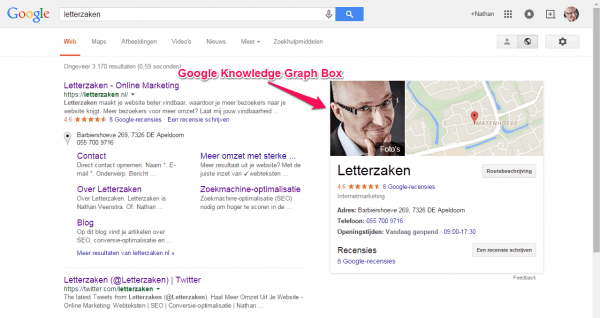
\includegraphics[width=\linewidth]{img/Google_Knowledge_Graph.png}
	\caption[Visualisatie Google Knowledge Graph]{Visualisatie Google Knowledge Graph}
	\floatfoot{	Source: https://letterzaken.nl/begrippenlijst/google-knowledge-graph-box/}
	\label{fig:GoogleKnowledgeGraphVis}
\end{figure}


Sinds de uitvoering van de Google Knowledge Graph is deze term zelf bekend geraakt, en wordt deze algemeen gebruikt voor het representeren van kennis die gebaseerd is op een graaf.

Binnen de informatica worden knowledge graphs ook wel ontologieën genoemd, dit soort graaf houdt eigenlijk een verzameling van onderling gelinkte objecten en feiten bij, die zowel door mensen als computers eenvoudig en ondubbelzinnig te begrijpen zijn.   

Op dezelfde manier dat Google zijn eigen Knowledge Graph gebruikt om haar zoekresultaten te verbeteren, kan er ook een graaf opgesteld worden voor andere toepassingen zoals een webshop. In de context van e-commerce toepassingen kan deze graaf gebruikt worden om relaties tussen producten te ontdekken. 

Aangezien het doorlopen van een graaf zoals eerder besproken zeer snel kan gebeuren, is dit een ideale troef om gepersonaliseerde zoekresultaten te kunnen aanbieden aan gebruikers. \autocite{E-CommerceKnowledgeGraph}

Door middel van een graaf kan geanalyseerd worden welke soorten producten vaak samen gekocht of bekeken worden, alsook ontdekken in welke producten gebruikers van e-commerce toepassingen geïnteresseerd zijn. Op basis hiervan kunnen aanbevelingen berekend en aan de gebruiker getoond worden. 
\newpage
In de context van aanbevelingssystemen worden knowledge graphs vooral gebruikt om extra kennis toe te voegen aan een graaf met relaties tussen klanten en producten, waardoor er onderling meer connecties kunnen gelegd worden tussen klanten en producten, hierdoor zijn de mogelijkheden voor aanbevelingen plots enorm veel groter.
 
Het cold-start probleem dat eerder bij het puntje aanbevelingssystemen besproken werd, wordt hier ook deels mee opgelost. Als er weinig relaties zijn tussen klant en product, of in het geval van een cold-start zelfs geen, kan de knowledge graph, die kennis heeft over de producten en hoe populair deze zijn, hier een handje bij toesteken om toch succesvol aanbevelingen aan de gebruiker te bieden.

In het onderzoek van \cite{Grad-Gyenge2015} wordt een model voorgesteld waar attributen van bijvoorbeeld een persoon of een film wordt voorgesteld als een extra knoop in een graaf. Zo kunnen films gelinkt worden aan genres, jaar van release, acteurs, etc. en personen kunnen gelinkt worden aan een leeftijd, geslacht, locatie, etc.
Zo kunnen er bogen in de graaf toegevoegd worden die personen met bijvoorbeeld dezelfde interesses en leeftijd groeperen. 

Het is ook een mogelijkheid om gewichten toe te kennen aan deze relaties (bogen), zodat bijvoorbeeld interesse in genres harder doorweegt dan gelijkaardige leeftijd wanneer er een verband gelegd wordt tussen twee personen, op deze manier kunnen de aanbevelingen op maat gegenereerd worden voor andere toepassingen, zoals e-commerce, waar in sommige sectoren leeftijd misschien een belangrijkere relatie is dan regio.

\subsection{Neo4j}
\label{sec:Neo4j}

Er bestaan verschillende platformen voor SQL en relationele databanken, bijvoorbeeld Microsoft SQL Server, MySQL, Oracle, etc.
  
Zo zijn er ook verschillende platformen voor de hierboven beschreven NoSQL databanken, afhankelijk van welk type databank gezocht wordt. Neo4j is een van de meer bekende platformen voor graph databanken, dit platform zal gebruikt worden in dit onderzoek.

Walmart maakt gebruik van Neo4j om de aanbevelingen voor hun klanten op hun online webservices te optimaliseren \autocite{neo4jWalmart2014}. Zij gebruiken dit omdat graph databanken zeer snel over een gebruiker zijn koophistorie kunnen traverseren, en ook direct nieuwe mogelijke interesses kunnen halen uit het gedrag van de gebruiker. Daarmee wordt bedoeld dat er in real-time nieuwe connecties worden gelegd tussen de gebruiker en de producten, en hij de nieuwe aanbevelingen meteen zal zien, en niet enkele dagen of uren later. Er wordt dus historische data gematcht met real-time data, hier blinkt Neo4j in uit. 

Neo4j maakt dus gebruik van wiskundige grafen om data weer te geven samen met hun onderlinge relaties. Een graaf kan gericht of ongericht zijn, ongericht wil zeggen dat er geen richting is waarin de relaties lopen, dus deze zijn onderling uitwisselbaar. 

Een gerichte graaf is dan een graaf waarbij de relaties in een specifieke richting lopen, zoals volgers op Twitter: Persoon A volgt persoon B, maar persoon B volgt niet persoon A. Voor een voorbeeld van hoe een graaf voor Twitter er in simpele vorm uit zou kunnen zien, is zichtbaar in Figuur \ref{fig:TwitterGraphExample}

\begin{figure} [hbt!]
	\centering
	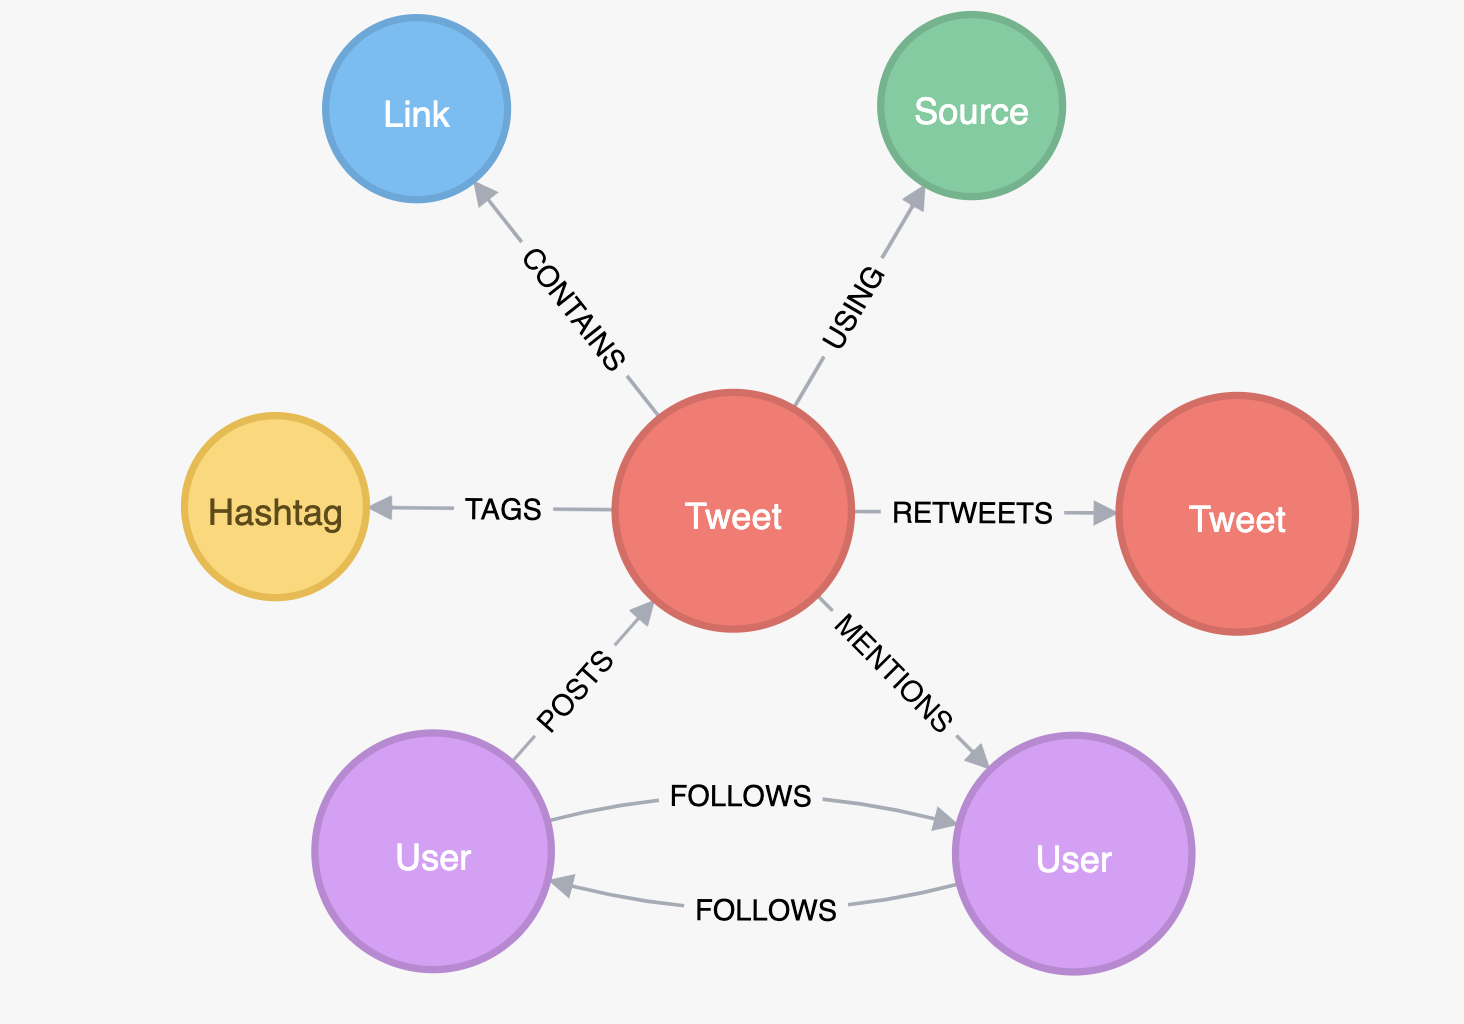
\includegraphics[width=\linewidth]{img/twitter_graph}
	\caption[Visualisatie gerichte graaf - netwerk]{Visualisatie gerichte graaf - netwerk}
	\floatfoot{	Source: http://network.graphdemos.com/}
	\label{fig:TwitterGraphExample}
\end{figure}

\newpage
\subsubsection{Performantie}
\label{subsubsec:Performantie}

In hoofdstuk één van het boek 'Neo4j in Action' \autocite{Vukotic2014} wordt een onderzoek gedaan naar de snelheid van het uitvoeren van bepaalde query's zoals 'zoek vrienden van vrienden' op een dataset. De resultaten hiervan wijzen erop dat graph databanken beduidend sneller zijn in het traverseren van een graaf, bijvoorbeeld voor het zoeken op een bepaalde diepte vanaf een startpunt.

Het experiment bestaat eruit 'vrienden van vrienden' op te halen uit een databank, dit in zowel Neo4j als MySQL. De databank bestaat voor beide platformen uit 1 000 000 gebruikers, \textit{Execution Time} wordt uitgedrukt in seconden per 1000 gebruikers.

In Tabel \ref{tab:Neo4j - MySql Comparison} worden de resultaten van dit experiment samengevat. De \textit{Depth} slaat hier op hoeveel vrienden een persoon van een andere persoon verwijderd zal zijn, voor een diepte drie is dit dus 'vrienden van vrienden van vrienden'.

	\begin{table}
		\centering
		\begin{tabular}{|l|l|l|}
			\hline
			Depth & Execution Time - MySQL                                & Execution Time - Neo4j \\ \hline
			2     & 0.016                                                 & 0.010                  \\ \hline
			3     &  30.267 & 0.168                  \\ \hline
			4     & 1,543.505                                             & 1.359                  \\ \hline
			5     & Not Finished in 1 Hour                                & 2.132                  \\ \hline
		\end{tabular}
	\caption{\label{tab:Neo4j - MySql Comparison} Source: https://neo4j.com/news/how-much-faster-is-a-graph-database-really/}
	\end{table}


Uit deze resultaten wordt al snel duidelijk dat Neo4j drastisch beter presteert bij het zoeken binnen netwerken van entiteiten waar veel connecties tussen voorkomen, wat nogmaals bevestigd dat voor dit soort use-cases, graph databanken de beste keuze zijn.



\section{Wat is ElasticSearch?}
\label{sec:wat is ElasticSearch?}

Elasticsearch op zichzelf is eigenlijk een zoek- en analyse-engine die data kan analyseren, of dit nu nummers, tekst, gestructureerd of ongestructureerd is. 

Elasticsearch is een component van de Elastic stack, ook wel ELK-Stack genoemd. Dit staat voor Elasticsearch, Logstash en Kibana. Logstash wordt gebruikt om data te verwerken uit meerdere bronnen en te versturen naar Elasticsearch. Kibana is een tool om de gebruikers een visueel beeld te geven van de data in de vorm van grafieken of tabellen.

Data wordt in Elasticsearch opgeslagen als een document in JSON-formaat in een index. Aangezien dit een zoekmachine is, is Elasticsearch dus gespecialiseerd in het zoeken van data, bijvoorbeeld een query om alle producten op te halen waar het woord 'switch' in voorkomt zal zeer snel resultaten opleveren.  

\newpage
Elasticsearch ondersteunt ook meerdere methodes voor het zoeken, eentje ervan is zoals hierboven beschreven het zoeken op een stukje tekst, waarbij alle documenten geretourneerd worden waar de tekst in een van de velden voorkomt, dit wordt tekst-gebaseerd zoeken genoemd.  Hieronder enkele voorbeelden van zoekmethodes:  

De zoekmethode die hier als voorbeeld genomen werd maakt gebruik van de parameter \textit{query\textunderscore string}. Als een van de velden van een document overeenkomt met de ingevoerde tekst, zal dit document in de lijst van resultaten terechtkomen.

\begin{lstlisting}[caption={Tekst-gebaseerd zoeken: Query om een simpele zoekopdracht uit te voeren met de term 'deodorant'}]
{
	"query" : 
	{
		"query_string": 
		{
			"query": "deodorant"
		}
	}
}
\end{lstlisting}

Er kan ook op specifieke termen gezocht worden via \textit{term}. Daarbij kan dan gespecificeerd worden welk veld moet overeenkomen met de ingevoerde tekst. 
Indien men wil zoeken op meerdere termen, kan de parameter \textit{term} vervangen worden door de parameter \textit{terms}, en zal er een array mee moeten gegeven worden als input in plaats van 'Audio' 

\begin{lstlisting}[caption={Tekst-gebaseerd zoeken: Query om een simpele zoekopdracht uit te voeren waar de categorie van het product overeen komt met 'Audio' }]
{
	"query" : 
	{
		"term": 
		{
			"category": "Audio"
		}
	}
}
\end{lstlisting}

Een andere manier om te zoeken op basis van tekst is \textit{match}. Hierbij worden alle woorden van alle velden van een document bekeken, en wordt er een score toegekend voor elke keer dit woord in het document voorkomt, op deze manier zullen resultaten waarbij dit woord het vaakst voorkomt, bovenaan in de lijst van resultaten terechtkomen. 
\newpage
\begin{lstlisting}[caption={Tekst-gebaseerd zoeken: Query die de resultaten sorteert op basis van hoe vaak het woord 'accepted' voorkomt in het veld 'message' van een document }]
{
	"query" : 
	{
		"match": 
		{
			"message": "accepted"
		}
	}
}
\end{lstlisting}

Als men wil zoeken binnen een bepaalde prijsklasse, bijvoorbeeld tussen 30 en 50 euro, kan dit met de parameter \textit{range}, bijvoorbeeld met volgende query:

\begin{lstlisting}[caption={Bereik zoeken: Een query om alle documenten op te halen waarbij het veld 'price' tussen 30 en 50 ligt}]
{
	"query" : 
	{
		"range": 
		{
			"price": {
				"gte": 30,
				"lte": 50
			}
		}
	}
}
\end{lstlisting}


Het is ook mogelijk om query's te combineren, dit kan verwezenlijkt worden door het gebruik van een \textit{bool query}. De parameters die hieronder gebruikt kunnen worden zijn:

\begin{itemize}
	\setlength\itemsep{1em}
	\item \textit{``must``} : De meegegeven waarde moet in het document voorkomen en de score van deze query zal meetellen voor de totale score. Dit is een strikte voorwaarde, als hier niet aan voldaan wordt zal het document niet opgenomen worden in de resultaten.	
	\item \textit{``filter``} : De meegegeven waarde moet in het document voorkomen. De score van deze query zal niet meetellen voor de totale score. Alle documenten die niet aan de voorwaarden van de filter voldoen, zullen net zoals bij 'must' niet opgenomen worden in de resultaten.	
	\item \textit{``should``} : Als de gegeven waarde voorkomt in het document, zal de score van het document verhoogd worden, maar dit is geen strikte voorwaarde. De parameter \textit{``minimum\textunderscore should\textunderscore match``} geeft aan aan hoeveel voorwaarden voldaan moet worden om het document op te nemen in de resultaten. De \textit{``boost``} parameter laat toe bepaalde overeenkomsten een hogere score te laten genereren.
	\item \textit{``must\textunderscore not``} : Het omgekeerde van 'must'. De meegegeven waarde mag niet voorkomen in het document. De score voor deze query zal ook niet meetellen. 
\end{itemize}

\begin{lstlisting}[caption={Combineren: Voorbeeld van een 'bool' query}]
{
	"query" : 
	{
		"bool": 
		{
			"must": {
				"term" : { "name" : "Kim" }
			},
			"must_not": {
				"term": { "lastname" : "Johnson" }
			},
			"filter": {
				"term": { "gender" : "female" }
			},
			"should" : [
				{
					"range" : {
						"age" : { "gte" : 20, "lte" : 30 }
					}
				},
				{
					"range" : {
						"height" : { "gte" : 150, "lte" : 170 } ,
						"boost" : 3
					}
				},
				{
					"term" : { "country" : "Belgium" }
				},
			],
			"minimum_should_match": 2
		}
	}
}
\end{lstlisting}
 
Bovenstaande query zal alle documenten retourneren waar: 
\begin{itemize}
	\setlength\itemsep{.3em}
	\item De voornaam 'Kim' is
	\item De achternaam NIET 'Johnson' is
	\item Het geslacht 'female' is.
\end{itemize}

En er aan minstens twee van deze drie voorwaarden voldaan wordt: 
\begin{itemize}
	\setlength\itemsep{.3em}
	\item De leeftijd tussen 20 en 30 jaar is
	\item De lengte tussen 150 en 170 is
	\item Het land 'België' is.
\end{itemize}


\newpage
In Elasticsearch is het dus mogelijk gewichten toe te kennen aan de resultaten van een zoekopdracht, zo kunnen meer relevante resultaten hoger in de lijst staan, dit is een belangrijke factor in dit onderzoek, namelijk of deze technologie gebruikt kan worden in E-Commerce toepassingen.

Een alternatieve en meer uitgebreide manier om scores toe te kennen aan resultaten is via een \textit{``function\_score``}. Het bovenste deel van deze query (\textit{``query``}) zal bepalen welke documenten opgenomen moeten worden, en het onderste deel ( \textit{``functions``}) zal een lijst van functies vormen. 

Aan de hand van deze functies zal een score voor een resultaat worden berekend. Aan elk van deze functies kan een gewicht (\textit{``weight``}) worden toegekend om bepaalde overeenkomsten meer te laten doorwegen dan andere en deze dus een hogere score toe te kennen.

Er komen nog twee extra parameters kijken bij deze functies, namelijk \textit{``score\_mode``} en \textit{``boost\_mode``}. Elk document dat wordt opgehaald zal een score toegewezen krijgen. 

De parameter score\_mode bepaalt hoe de scores  van deze functies gecombineerd worden. Mogelijke opties hiervoor zijn \textit{``multiply``}, \textit{``sum``}, \textit{``avg``}, \textit{``first``}, \textit{``max``}, en \textit{``min``}

De parameter boost\_mode bepaalt hoe de score van de query en de functies gecombineerd moet worden. Mogelijke opties hiervoor zijn: \textit{``multiply``}, \textit{``replace``}, \textit{``sum``}, \textit{``avg``}, \textit{``max``}, en \textit{``min``}.

De meeste opties verklaren zichzelf, \textit{``replace``} zal de score die toegekend werd aan het document bij het ophalen ( \textit{``query``}) overschrijven door de score die berekend werd door de functies. 

Hieronder een voorbeeld van een function\_score query waar alle documenten opgehaald worden, daarna zal er een score van 4 toegekend worden aan de documenten indien 'name' overeenkomt met 'Kim', en een score van 2 indien 'age' overeenkomt met '23'.

De scores van deze functies zullen worden opgeteld, en het resultaat hiervan zal de score die toegekend werd aan het resultaat bij het ophalen van het document overschrijven. 

\newpage
\begin{lstlisting}[caption={Scoring: voorbeeld van een function\_score query}]
{
	"query" : {
		"function_score" : {
			"query" : { "match_all" : {} },
			"boost" : 2,
			"functions" : [
				{
					"filter" : { "match" : { "name" : "Kim" } },
					"weight": 4
				},
				{
				"filter" : { "match" : { "age" : 23 } },
				"weight": 2
				}
			],
			"score_mode" : "sum",
			"boost_mode" : "replace"
		}
	}
}
\end{lstlisting}

De \textit{``script\_score``} functie laat toe om een score voor een document te berekenen aan de hand een van de waarden van de velden in het document.

Onderstaande query zal alle documenten ophalen waarbij het veld 'naam' overeenkomt met 'Kim', en zal een score berekenen op basis van de lengte van deze persoon. In dit geval (300 - lengte) zal een lagere waarde voor dit veld resulteren in een kleinere score.

\begin{lstlisting}[caption={Scoring: voorbeeld van een script\_score query}]
{
	"query" : {
		"script_score" : {
			"query" : {
				"match" : { "name" : "Sasha" }
			},
			"script": {
				"
				height = doc['length'].value;
				return 300 - length;
				"
			}
		}
	}
}
\end{lstlisting}

Decay functies kunnen gebruikt worden om de score van een document aan te passen naar gelang een opgegeven veld afwijkt van een bepaalde waarde. Dit is gelijkaardig aan de 'range' query, waar met intervallen zou kunnen werken, maar loopt geleidelijk mee naargelang de afstand tussen de waarde van het veld en de opgegeven waarde groter wordt. 
\newline

Er zijn drie mogelijke decay functies, namelijk \textit{``linear``}, \textit{``exp``}, en \textit{``gauss``}. De velden die hierbij horen zijn:

\begin{itemize}
	\item \textit{``origin``} : Het startpunt voor het berekenen van de afstand. De waarde hiervan moet numeriek, een datum of een geo-punt zijn.
	\item \textit{``scale``} : Het verschil dat nodig is om de score te doen afnemen met de waarde aangegeven door de decay.
	\item \textit{``offset``} (Optioneel):  Als deze waarde gedefinieerd wordt, zal de decay functie enkel berekend worden als de afstand groter is dan deze waarde. Default is 0.
	\item \textit{``decay``} (Optioneel): Geeft aan met welke waarde de score van een document moet afnemen. Default is 0.5
\end{itemize}


\begin{lstlisting}[caption={Decay: voorbeeld van een decay functie}]
{
	"query" : {
		"function_score" : {
			"exp" : {
				"date" : {
					"origin": "2013-09-17",
					"scale" : "10d",
					"offset" : "5d",
					"decay" : 0.5				}
			}
		}
	}
}
\end{lstlisting}

De bovenstaande query zal de score van een document laten afnemen met 0.5 naar gelang de waarde van het veld 'datum' verder ligt van de opgegeven waarde (2013-09-17). De waarde zal niet afnemen indien deze binnen de 5 dagen verwijderd ligt van de opgegeven waarde.

 In het artikel van \autocite{Vavliakis2019} wordt beweerd dat het systeem dat zij implementeerden op een performante manier de gewenste resultaten gaf, alsook dat dit een oplossing kan zijn voor real-time zoekopdrachten in commerciële toepassingen. Dit sluit dus al uit dat Elasticsearch geen oplossing zou kunnen bieden voor onze onderzoeksvraag.
 
 \newpage
\section{Filter Bubble}
\label{sec:Filter Bubble}

Een filter bubble, ook wel informatieluchtbel genaamd, is een gevolg van het personaliseren van zoekopdrachten. Personalisatie is het proberen bepalen welke zaken een gebruiker zou willen zien, aan de hand van een algoritme. 

Een filter bubble betekent dat door deze personalisatie, bijvoorbeeld geen producten zal zien die hem niet interesseren, in dit geval is dat een voordeel. Als we kijken in de context van controversiële onderwerpen, zorgt deze bubbel ervoor dat de gebruiker eigenlijk geen informatie zal zien die niet bij zijn standpunt past, de gebruikers worden dus afgesloten in een luchtbel die bestaat uit enkel hun visie of standpunt.  \autocite{Pariser2011}

Pariser geeft als voorbeeld in zijn boek een scenario waar een gebruiker de zoekterm ``BP``invoerde, en resultaten kreeg in verband met investeringsnieuws over British Petroleum. Een tweede gebruiker gaf dezelfde zoekterm in en kreeg informatie over Deepwater Horizon als resultaat. Dit is dus een merkwaardig verschil.

Parser beweert dat het effect van de filter bubble negatieve gevolgen kan hebben voor de manier waarop mensen hun mening vormen, dit aangezien zij geen argumenten te zien krijgen die hun mening tegenspreken.


De relevantie van dit fenomeen voor dit onderzoek valt op het feit dat bij de Content Based algoritmen die eerder besproken werden, we met een gelijkaardig probleem te maken hadden. Bij deze aanbevelingssystemen kan er overspecialisatie optreden, waardoor de gebruiker enkel producten aanbevolen krijgt die reeds gezien zijn, of té gelijkaardig zijn, en er dus geen nieuwe verrassende producten aangeboden worden.

\section{GDPR}
\label{sec:GDPR}

Op 25 mei 2018 is de \textit{General Data Protection Regulation} (GDPR) ingevoerd. Dit is een verzameling van regels die bestaat om de persoonlijke data van inwoners van de EU te beschermen. Met persoonlijke data wordt verwezen naar data die direct of indirect kan gelinkt worden aan een persoon, het gaat hierbij over data zoals IP-adressen en cookies. 

Onder deze regulatie is het verplicht voor bedrijven om toestemming te vragen aan hun gebruikers om persoonlijke data te mogen opslaan en verwerken. Meestal gebeurt dit in de vorm van een knop waar de gebruiker op moet klikken om cookies toe te staan, en zelfs daar kan de gebruiker soms nog zelf enkele opties aanvinken over welke data hij wil vrijgeven aan het bedrijf. \autocite{Goddard2017}

Enkele onderdelen die van belang zijn voor e-commerce toepassingen worden verder besproken in de volgende hoofdstukken.

\subsection{Gegevensverwerking}
\label{subsec: Gegevensverwerking}

Bedrijven mogen onder deze regulatie niet zomaar eender welke persoonlijke gegevens van hun gebruikers verwerken. Er werden enkele regels opgesteld die bedrijven moeten volgen indien zij toch wensen om persoonlijke data te verwerken, en er moet aangetoond kunnen worden dat deze regels nageleefd en gerespecteerd worden. Deze regels zijn terug te vinden in artikel 5 van de GDPR, genaamd ``Beginselen inzake verwerking van persoonsgegevens`` \autocite{Article5GDPR2018}.

Het verwerken van persoonsgegevens moet rechtmatig, behoorlijk en transparant gebeuren. Dit wil zeggen dat er aan minstens één van de voorwaarden in Artikel 6 van de GDPR voldaan moet worden.
\begin{itemize}
	\item Een persoon geeft expliciet toestemming voor het verwerken van zijn gegevens.
	\item De verwerking is noodzakelijk in het kader van een wettelijke plicht of om de vitale belangen van een persoon te beschermen
	\item  De verwerking is noodzakelijk voor het algemeen belang of de uitoefening van het openbaar gezag
	\item De verwerking is noodzakelijk voor een gerechtvaardigd belang. 
\end{itemize}
\autocite{Article6GDPR2018}

De regulatie verplicht ook dat slechts het minimum aan persoonlijke data van een gebruiker wordt opgeslagen, en moet dus beperkt blijven tot de data die van belang is voor de doelen waarvoor die data gebruikt zal worden.

Als er wordt gesproken over transparantie, wil dit zeggen dat er geen twijfel mogelijk mag zijn over hoe de persoonlijke data van een gebruiker verwerkt wordt. Ook mogen enkel en alleen verwerkingen uitgevoerd worden waar een gebruiker mee instemt.


\subsection{Rechten van de gebruikers}
\label{subsec: Rechten van de gebruikers}

Indien een persoon de persoonlijke data wenst op te vragen, verplicht de wetgeving rond GDPR  bedrijven om deze data, samen met andere informatie op te leveren, al dan niet in digitaal formaat.

Deze oplevering van persoonlijke data moet binnen een redelijke tijdspanne gebeuren, en er mogen dus geen onrealistische vertragingen plaatsvinden hierbij. Enige uitzondering hiervoor is wanneer een van de condities in Artikel 17, punt 3 van toepassing zijn. 

 Een volledige beschrijving van deze informatie is terug te vinden in Artikel 15 van de GDPR, ``recht van inzage van de betrokkene``. \autocite{Article15GDPR2018}

Een persoon heeft het recht om de persoonlijke data te laten wissen. Dit moet zonder onredelijke vertraging kunnen gebeuren, tenzij een van de uitzonderingen in Artikel 17, punt 3 van toepassing zijn.

Persoonlijke gegevens moeten gewist worden wanneer: 

\begin{itemize}
	\item Deze gegevens niet langer nodig zijn voor de doelen waarvoor deze verzameld zijn.
	\item De betrokken persoon trekt zijn toestemming voor de verwerking in.
	\item De betrokken persoon maakt bezwaar tegen de verwerking.
	\item De gegevens zijn onrechtmatig verwerkt.
\end{itemize}
\autocite{Article17GDPR2018}

De volledige lijst staat beschreven in Artikel 17 van de GDPR.

De details van deze wetgeving worden niet verder uitgewerkt of toegepast in deze scriptie, aangezien dit te ver afwijkt van het onderzoek. De informatie die hier te vinden is, is louter een algemene conclusie die tracht de nodige aandachtspunten in verband met de GDPR in kaart te brengen.

\subsection{Effect van de GDPR op e-commerce}
\label{subsec: Effect van de GDPR op e-commerce}

In het geval van e-commerce toepassingen zijn de voorwaarden over wettelijke plicht of een gerechtvaardigd belang niet van toepassing. Indien een e-commerce website de data van een gebruiker zou willen verwerken, zal deze expliciete toestemming moeten vragen aan de gebruiker.

Een gebruiker moet op transparante wijze ingelicht worden over hoe zijn gegevens verwerkt zullen worden, en dus voor welke doeleinden deze gegevens zullen dienen. Er zal ook geen data mogen bijgehouden worden die niet gebruikt wordt. 

Een evidente keuze hiervoor is om gebruik te maken van cookies, en hiervoor expliciete toestemming te vragen aan de gebruiker. Er zal dan een privacybeleid moeten worden opgesteld waar in duidelijke en heldere taal beschreven staat welke data verwerkt zal worden, en voor welke doeleinden. 

\begin{figure} [h!]
	\centering
	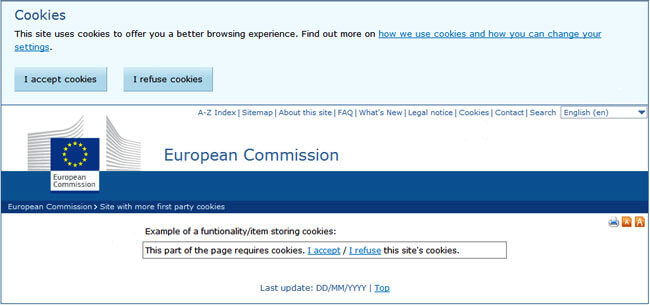
\includegraphics[width=\linewidth]{img/180321-EU-Cookie-Consent-Examples}
	\caption[Voorbeeld Cookie Consent]{Voorbeeld Cookie Consent}
	\floatfoot{	Source: https://www.freeprivacypolicy.com/blog/cookie-consent-examples/}
	\label{fig:CookieConsentExample}
\end{figure}



Er mogen geen dubbelzinnigheden of onduidelijkheden terug te vinden zijn, en er mag geen informatie achterwege gelaten worden. Ook informatie over welke data naar derden gestuurd wordt, en voor welke redenen moet hier duidelijk vermeld worden.





